
\documentclass[a4paper,12pt]{article}

%% Language and font encodings
\usepackage[english]{babel}
\usepackage[utf8]{inputenc}
\usepackage[T1]{fontenc}

%% Sets page size and margins
\usepackage[a4paper,top=3cm,bottom=2cm,left=3cm,right=3cm,marginparwidth=1.75cm]{geometry}

%% Useful packages
\usepackage{amsmath}
\usepackage{amssymb}
\usepackage{graphicx}
\usepackage{listings}
%\usepackage{algorithmic}
%\usepackage{algpseudocode}% http://ctan.org/pkg/algorithmicx
\usepackage{float}
\usepackage[colorinlistoftodos]{todonotes}
\usepackage[colorlinks=true, allcolors=blue]{hyperref}
\usepackage{nomencl}
\usepackage{bm}
\usepackage{titling}
\usepackage{gensymb}
\usepackage[]{algorithm2e}
\usepackage{placeins}
\usepackage{subfig}
\setlength{\parindent}{0pt}
\numberwithin{equation}{section}
\usepackage{subcaption}
\usepackage{mwe}
\usepackage{floatrow}
\usepackage[nottoc]{tocbibind}
% Table float box with bottom caption, box width adjusted to content

\newdimen\prevdp
\def\leftlabel#1{\noalign{\prevdp=\prevdepth
   \kern-\prevdp\nointerlineskip\vbox to0pt{\vss\hbox{#1}}\kern\prevdp}}
\def\Sum{\sum\limits}

\title{Applications of Alternative Measurements to Meta-heuristic Based Clustering Models}
\author{Alex Wong}
\begin{document}
\maketitle
\begin{abstract}
We will discuss the application of different norms on clustering algorithms.  These different norms produce different measures of similarities between points assigned to the same cluster.  We explore modifications to the classic KMeans algorithm, as well as simulated annealing and genetic algorithms for clustering.  Computational results from various public domain data sets are used for comparison.  We also present some thoughts on extensions of these studies.
\end{abstract}
\section{Introduction}
Clustering is a common approach to classification and predictions with applications to machine learning and artificial intelligence. Clustering models have been classified as form of unsupervised learning, which is a branch of machine learning algorithms that involves working with unlabeled data to provide insights. The goal with clustering models is to partition the data into k groups such the dissimilarity is minimized for all partitions; therefore within a given partition all the points are relatively similar to each other. In most cases, a center is chosen for the cluster that describes its respective members and the cost function is chosen with respect to a distance metric.\\

Clustering is a widely studied problem with many different techniques but the majority do it with respects to the $\ell_2$ norm. For our analysis, we will be using a combination of deterministic and meta-heuristics to discuss the effects with the metric spaces $\ell_1$ and $\ell_\infty$. In Section \ref{sec:clustering_def}, we will be discussing the general clustering problem with more information provided for the deterministic and meta-heuristic case provided in Sections \ref{sec:deterministic} and \ref{sec:metaheuristic} respectively. Next, we will discuss implementation details with respects to the introduced heuristic in Section \ref{sec:implementation}. Lastly, the results of our finding are presented in Section \ref{sec:results}.

\subsection{Literature Review}
This section will primarily focus on 3 alternative forms to clustering. Those include Bilinear KMedian, Simulated Annealing, and Genetic Algorithms.\\ 

The first paper, we looked at from INFORM Journal of Computing, where the article discussed how to convert data mining models in to the realm of mathematical programming\cite{bradley_fayyad_mangasarian_1999}. In particular, the model We are going to be concentrating on was an adaptation of KMeans into the scope of Linear Programming. The article goes on to explain that because $\ell_2$ is not feasible in a linear programming system that an alternative norm must be used. Likewise clustering cannot be done with a singular linear program because there is two underlying sub problems that when combined make a quadratic system.  This is where the author decides to use the concept of Bilinear Programming to decouple the problems into two independent linear programs that would feed each other with the data. \\

Next, the simulated annealing paper by Merendino \cite{Merendino}, looked at ways of resolving the problem of getting caught in a local minimum for the system. It did outline the general principals of simulated annealing and it tried to improve on how to build the next state of the system.  Likewise, this paper primarily focused on trying to use the $\ell_2$ distance metric when resolving the local minimum problem.  \\

Lastly, the paper about genetic algorithms by Bandyopadhyay \cite{bandyopadhyay_maulik_2002} outlined a lot of the core features, such as how to model the system. It did leave out some information about how to do some of the core feature of genetic algorithms but it did describe relative fitness with respects to $\ell_2$. 

\section{Background}
 In this section we will primarily focus on defining the problem along with a brief description of each algorithm or meta-heuristic. Before we can address and define clustering, we first must describe how it gets quantified. 
\subsection{Metric Space}
Norms are forms of doing measurements in vector spaces. The norms in this case refers to how the distance function is computed for each space. Every norm is going to start from the same starting point of two n-dimensional vectors in $\mathbb{R}^n$.\\

Let $v_1$ and $v_2$ be vectors in  $\mathbb{R}^n$.
\begin{equation}
\textbf{x} = v_1-v_2
\label{eq:diff}  
\end{equation}

\subsubsection{$\ell_2$ : Euclidean Distance}
The Euclidean distance is the most common form of the distance function. It calls for square rooting the sum of the squares. Thus in $\mathbb{R}^2$ it looks like the common distance function of $\sqrt{(x_1-x_2)^2+(y_1-y_2)^2}$. In the general case it can be described as the following. \\

In the general case, continuing from \eqref{eq:diff}, for $\ell_2$ will look like the following for the distance function.

\begin{equation}
    distance =  \|v_1- v_2\|_2 = \sqrt{\sum_{k=1}^n (v_{1,k} - v_{2,k})^2}
\end{equation}
The issue with the Euclidean distance is that it can exaggerate already bad dimension because of the squaring term in the radical. 

\subsubsection{$\ell_1$ : Manhattan Distance}
The $\ell_1$ norm can be described as the sum of the absolute values for every element in the vector. It is also describe as the Manhattan distance because movement from one location to another in $\mathbb{R}^2$ will resemble the movements along city blocks. With the Manhattan distance all, $x_k$, difference are weighted equally with respect to each other unlike in the case of $\ell_2$. With Euclidean distance, larger $x_k$ are then made larger to show the magnitude on the result. \\

In the general case, continuing from \eqref{eq:diff}, for $\ell_1$ will look like the following for the distance function.
\begin{equation}
    distance =  \|v_1- v_2\|_1 = \sum_{k=1}^n |v_{1,k} - v_{2,k}|
\end{equation}

\subsubsection{$\ell_\infty$ : Supremum Distance}
The $\ell_\infty$ norm is maximum among the absolute values for all $x_k$. This distance metric focuses on the fact that a resulting vector can only be defined by how far its furthest dimension is. It is important in the case where we know in $x_k$ there exist a value of $\gamma$ by which all other values in $\textbf{x}$ are bounded by; thus $\gamma$ would be the distance. Even if the $v_2$ was approaching $v_1$ in all dimension except for $x_k$ the value would still be $\gamma$ signifying the other dimensions can do anything with respects to the $x_k$ dimension. \\

In the general case, continuing from \eqref{eq:diff}, for $\ell_\infty$ will look like the following for the distance function.
\begin{equation}
    distance =  \|v_1- v_2\|_\infty = \max_k |v_{1,k} - v_{2,k}|
\end{equation}
\subsection{Clustering Definition} \label{sec:clustering_def}
Clustering as stated earlier is the problem of identify groups in the data such that member of each group are similar to each other. In reality it is nearly impossible to find groupings that are perfectly similar to each other so instead groups just try to minimize their respective errors. In the case of the KMeans algorithm it would be minimizing the error between a point $p_i$ and its respective centroid $c_j$. In the most common case for clustering the euclidean distance ($\ell_2$) is used as the error metric. As for the general case the square errors will look like the follow.  
\begin{equation}
SE_j = \sum_i \|(x_i- c_j) \| 
\end{equation}
In this case, $x_i$ are all the points assigned to that particular center $c_j$ and the norm is some arbitrary norm. Since we have now found a way to quantify the error for a particular groups lets apply this technique to all groups. Therefore having SSE= $\sum\limits_{j=1}^{k} SE_j$ where $k$ is the number of desired groups to be formed. The overall objective is to minimize the SSE, thus each subsequent SE for each grouping is minimized. 

\subsection{Deterministic Clustering} \label{sec:deterministic}
The deterministic-based clustering models utilize the computational model described by a deterministic Turing machine. The purpose of using a deterministic based model is to ensure that any given input always produce the same output. This implies that there exist no randomness in the processes when producing the answer and it is always repeatable. \\

Some of the classical deterministic algorithms for clustering that are discussed in this paper is KMeans Clustering and Bilinear KMedians Clustering. 

\subsubsection{KMeans Clustering}
KMeans clustering as mentioned earlier is an NP-Hard Problem\cite{mahajan_nimbhorkar_varadarajan_2009}. It has two functions either points can be assigned to a cluster or the cluster center can be updated to reflect the points assigned to that particular group. This will be repeated until the updates of the assignments and the recentering of the clusters don't adjust anything.  \\

\begin{algorithm}[]
 Select K points as the initial centroids\;
\While{The centroid don't change}{
    Form K clusters by assigning all points to the closest centroid as measured by $\ell_2$\\
    Recompute the centroid of each cluster
 }
\caption{KMeans Clustering Algorithm}
\end{algorithm} 
\newline
The assignment of points to a cluster will be resolved with a greedy nearest neighbors approach. Given a point $i$ it will compare its respective distance across all known cluster centroids and select the closest one for assignment. The recentering or recomputation of the center is done by looking at all assigned points to cluster $k$ and averaging each dimension. The KMeans algorithm will eventually create a system that is convergent to some local minimum after some arbitrary amount of iterations. It is very typical to see KMeans clustering done with respect to the $\ell_2 $ norm for calculating the distance between the centers and its respective point.

\subsubsection{Bilinear KMedians Clustering}
Bilinear KMedians clustering is a modification of the classical kmeans cluster method expect the recentering is done with respects to the median value for each dimension and the distance is done with respects to $\ell_1$ and $\ell_\infty$ norms for my purposes. \\

Since it is not feasible to decouple the assignments of the points to the centroids and the centroids location in space, a bilinear approach is needed to solve this problem. Using the bilinear approach certain aspect of the linear program are held constant while other are being solved for. Those result are then shipped to the other linear program and then resolved. Thus, we have two different linear programs that have circular dependency on each other. The termination condition for this approach is to continue until the algorithm sees the same results twice in a row after each solve.  
\begin{figure}[H]
    \centering
    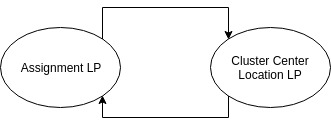
\includegraphics[scale = 0.55]{images/bilinear.jpeg}
    \caption{Bilinear Flow Diagram}
    \label{fig:bilinear_flow}
\end{figure}
The Assignment linear program works by assuming the locations of the centroids to be fixed in space and therefor will solve for best assignment between points and centroids. The Cluster Center linear program works by fixing the assignment between points and centroid labels. Thus, it will solve for new centroid location that are more indicative of the assignments. The circular flow will occur when the Assignment linear program will send off new assignment labels for the points into the Cluster Center location linear program which will compute new centroids given the assignments. Further discussion on this model will be left for the implementation discussion in Section \ref{sec:bilinear_imp}.

\subsection{Meta-heuristic Clustering Methods} \label{sec:metaheuristic}
Meta-heuristic based clustering methods are clustering algorithms that utilize a stochastic computation model and thus a stochastic Turing machine. In this case instead of using the classical Turing machine which is built with respects to a deterministic model of computation where all movements are predictable. 
A stochastic Turing machine uses probability theory to decide in the state transitions of the system. \\ 

Typically meta-heuristics are used for partial search algorithms because identifying the total ordering would take too long. Such problems are in NP, meaning there currently does not exist any polynomial time algorithm to solve the problem with respects to the size of the inputs. Likewise, if the polynomial time algorithm has a very large run-time it is also applicable to use meta-heuristics. Another way to think about meta-heuristics based clustering is to think about finding the best solution to a system but instead find a good solution to the system.  

\subsubsection{Simulated Annealing}
This meta-heuristic is inspired by the physical process of heating and cooling a metal. As the metal is heated, the atoms of the metal are more malleable and can move more freely. But as the metal is cooled, it becomes more rigid and more difficult to change its respective state. \\

Simulated Annealing algorithm works by doing random movements or adjustments to the state relative to a global temperature of the system. In this algorithm improving adjustments are always accepted while non-improving changes are accepted with some probability relative to the temperature of the system. This can be explained from actual process of cooling metal because the metal should be more difficult to do a poor adjustment when it has cooled off. \\

This algorithm also calls for a cooling schedule. The cooling schedule reflects how the system adjusts its temperature. This includes but is not limited to the the starting temperature, $T_i$, the freezing or ending temperature $T_f$, and the change in temperate function. This function defines the step size for the cooling schedule. \\

Lastly, this meta-heuristic has two forms of determining the best state. In one case the best state is the final state after the freezing temperature is hit. This case can be described as where you end up is where you end up because it does not care about if at some other point it found a more optimal solution. The other case keeps track of the best overall state in the event the final state is worse. This case takes into account that a better state was found but the algorithm chose to move away from it. Further discussion of the algorithm and its details will be left for Section \ref{sec: sa_imp}.

\subsubsection{Genetic-based Algorithm}
This meta-heuristic comes from evolutionary biology, where genes and chromosomes describe the state of the system based on some relative fitness function. In a genetic-based algorithm there are some core functions that all models must employ those being crossover, mutation and selection of the genes. Using these basic functions, the idea is to generate an artificial natural selection environment where good sets of chromosomes describing the states are selected for further generations. \\

This is similar to what Charles Darwin observed in the Galapagos Islands with the tortoises. He observed that particular tortoises had a comparative advantage in feeding with certain features relative to others. The same can be said for the algorithm because a genetic algorithm starts with a gene pool. In this case, a gene pool represents a bunch of different states for a particular model and the relative fitness is the quantifier for each state. \\

Using the ideas of relative fitness, states will begin to intermingle to generate new states. This is akin to the creation of new generations in actual animals or plants. For instance, a botanist wants to create a new species and combine two plant species for their respective strengths. The chromosomes will cross and produce an offspring that constitutes the next generation.\\

The functions as mentioned earlier with crossover, selection and mutation can be thought of as mixing, selection of the best feature, and exploratory search respectively.  We will continue the discussion of how each of these function works in Section \ref{sec:ga_imp}.

\section{Implementation Details} \label{sec:implementation}
In this section, we will be discussing the implementation details of the deterministic and meta-heuristics algorithms presented. All the algorithms with the respective data were able to run on an x86\_64 computer with at most 32 GB of ram. All of these implementations required Python3 with additional packages from pypi, the python package index, including pandas, numpy, matplotlib, and sklearn.\\

Pandas was used for the maintaining and cleaning the data that was produced from each run. In some ways pandas is just a convenient way to work with csv files and perform simple queries on. Numpy was used because it offers a python based implementation for a lot of the linear algebra procedures that would come with Matlab.  Matplotlib was a convenient way to produce plots of the data in the tidyverse that will later be shown in Section \ref{sec:results} . Lastly, we used sklearn because it had an existing implementation of KMeans Clustering built in. 

\subsection{Bilinear KMedian Models}\label{sec:bilinear_imp}
The Bilinear models use the Gurobi Optimizer software and pyomo, the mathematical modeling language, for building the models. The work flow is to build the linear program in Python3 with pyomo and then hand off the model to the Gurobi Optimize . Since we are doing the analysis with respects to multiple norms there is going to be two different KMedian models, one for $\ell_1$ and another for $\ell_\infty$. \\

There is going to be some commonality between the two bilinear programs with the sets and the some of the nomenclature. In both cases there is going to be an assignment linear program where points are assigned to arbitrary centroids and a recentering linear program which is going to find the centroid relative to the assignments.

\subsubsection{$\ell_1$ Model}
The first linear program, we are going to discuss is the Assignment linear program. In this model we let $P$ be the set all points, $K$ be the set of all desired centroids and $D$ be the dimensionality of the system. The desired objective function is as follows with equation (\ref{eq:objective}).
 \begin{equation}
 \text{min} \quad \sum_{i \in P}\sum_{j \in K}\sum_{d \in D} (S^{+}_{i,j,d}+S^{-}_{i,j,d}) 
 \label{eq:objective}
\end{equation}
In equation (\ref{eq:objective}), $S^{+}_{i,j,d}$ and $S^{-}_{i,j,d}$ describes the amount of overshoot and undershoot the system is undertaking because both $S^{+}_{i,j,d}$ and $S^{-}_{i,j,d}$ are in the positive reals. The following three equations are the constraints for the $\ell_1$ bilinear clustering model. 
\begin{equation}
0=A_{i,j}\cdot(P_{i,d}-\boldsymbol{C_{j,d}})+(S^{+}_{i,j,d}-S^{-}_{i,j,d}) \qquad \forall i \in P, j\in K, d \in D
\label{eq:distance_computation}
\end{equation}
\begin{equation}
1\leq \sum_{i \in P} A_{i,j} \qquad \forall j \in K
\label{eq:nonsingular}
\end{equation}
\begin{equation}
1 = \sum_{j \in K} A_{i,j}  \qquad \forall i \in P
\label{eq:hard_assignment}
\end{equation}
The first constraint(\ref{eq:distance_computation}) describes the penalty for the assignment between a point and the centroid. We let $A_{i,j}$ be a binary variable that shows if there is an assignment between point $i$ and centroid $j$ and $P_{i,d}$ be point $i$'s  $d$th dimension. Lastly $C_{j,d}$ is to show is in bold because it signifies that this variable is fixed from the start of the linear program. The second constraint (\ref{eq:nonsingular}) is used to guarantee all cluster have at least one point to them. The last constraint (\ref{eq:hard_assignment}) enforces hard clustering because a point can only belong to one cluster. When this linear program is solved it will generate new set of assignment between points and fixed centroid locations. \\

The other linear program for the recentering can be expressed with same objective function,(\ref{eq:objective}) as before but the difference is in the constraint. 

\begin{equation}
0=\boldsymbol{A_{i,j}}\cdot(P_{i,d}-C_{j,d})+(S^{+}_{i,j,d}-S^{-}_{i,j,d}) \qquad \forall i \in P, j\in K, d \in D 
\label{eq:flex_centers}
\end{equation}
In this case as opposed to equation (\ref{eq:distance_computation}), $A_{i,j}$ is fixed and we are now solving for the centroids of the clusters. Thus the flow of variable in this bilinear model would be from centroids, $C_{i,j}$, solved with the recentering linear program. The results would then be used to start the assignment linear program with $C_{i,j}$ being fixed and producing a new set of $A_{i,j}$ which describes the assignments. This process would spin around in a circle until the assignment linear program or the recentering linear program repeated its respective results signaling a termination. 
 
\subsubsection{$\ell_\infty$ Model}
The $\ell_\infty$ model is very similar to the $\ell_1$ bilinear model except now the enforced norm is $\ell_\infty$.  For the assignment and recentering linear program, they both have the same optimization function as shown in equation (\ref{eq:inf_opt}).

\begin{equation}
 \textbf{min}  \quad \sum_{i\in P}\sum_{j\in K} Z_{i,j} 
 \label{eq:inf_opt}
\end{equation}
This equation works by minimizing the $Z_{i,j}$ which we refer to as the crush factor bound for all points and centroids.  There are 4 constraints for the assignment linear program. Those constraints would be as followed. 
\begin{equation}
0=A_{i,j}\cdot(P_{i,d}-\boldsymbol{C_{j,d}})+(S_{i,j,d}) \qquad \forall i \in P, j\in K, d \in D 
\label{eq:distance}
\end{equation}
\begin{equation}
-Z_{i,j} \leq S_{i,j,d} \leq Z_{i,j} \qquad \forall i \in P, j\in K, d \in D 
\label{eq:bounded}
\end{equation}
\begin{equation}
1\leq \sum_{i \in P} A_{i,j} \qquad \forall j \in K 
\label{eq:non_empty}
\end{equation}
\begin{equation}
1 = \sum_j A_{i,j} \qquad \forall i \in P
\label{eq:hard}
\end{equation}
In this linear program, equation (\ref{eq:distance}) is used to describe the clustering assignment with $C_{i,j}$ being fixed in space and points being assigned to clusters. The next equation (\ref{eq:bounded}) refers to if the slack variables, $S_{i,j,d}$, are within the bounds that we are trying to crush and minimize. The last two constraints (\ref{eq:non_empty}) and (\ref{eq:hard}) are just logical rule for how the assignment should proceed similar to constrains (\ref{eq:nonsingular}) and (\ref{eq:hard_assignment}) from the $\ell_1$ model. In this case these two constraints refer to no cluster can be have an empty set of assignments and for all points there can only exist one assignment, respectively. \\

The recentering linear program as mentioned shares the same optimization function (\ref{eq:inf_opt}) as the assignment linear program. It also uses constraint (\ref{eq:bounded}) to ensure that distance is calculated correctly for $\ell_\infty$. The only difference is in this constraint. 
\begin{equation}
0=\boldsymbol{A_{i,j}}\cdot(P_{i,d}-C_{j,d})+(S_{i,j,d}) \qquad \forall i \in P, j\in K, d \in D 
\label{eq:distance_alt}
\end{equation}
This is an adaption of the distance computation (\ref{eq:distance}) from the other linear program except now $A_{i,j}$ is fixed and $C_{j,d}$ is free to move. Like the $\ell_1$ case the termination condition is until this becomes trivial with the handoffs of the data.  
\subsubsection{Simple Optimization}
A simple optimization to these algorithms was removing the recentering linear program. Instead of using a linear program solver to decide on the new  $C_{j,d}$. We chose to extract the necessary data from the assignment linear program and using numpy just called the median function for each cluster. 

This greatly reduced the memory requirements because we would be running out of ram on 32 GB machine with both linear programs being built. We suspect because of the size of the data and the way points are treated in this model that the number of constraints grew psuedopolynomially with respects to the number of points, dimensions and clusters being formed. 

\subsection{Simulated Annealing}\label{sec: sa_imp}
We chose to use numpy for the majority of the implementation of this algorithm.  Some the details of the algorithm were left out when we previously introduced the problem that include the general flow of the algorithms and how are new states decided upon. For our purposes, we chose to do a pure random style of generations. In this case, we would select approximately 2/3 of the population to be reshuffled and then recompute the total error with respects to the new norm from the assignments. This algorithm works by thinking of the centroids as derivative of the assignments and the not the assignments being derivatives of the centroid location using the greedy nearest neighbor heuristic. \\

There is only one crucial portion of the Simulated Annealing algorithm and that is how to deal with worse states. As previously mentioned, better states are always accepted but worse states are accepted with some probability. In that case, we have $SSE_1$ and $SSE_2$ where $SSE_1 < SSE_2$ with $SSE_2$ being the new proposed state. Let $\Delta SSE = SSE_2 - SSE_1$ which describes how much worse the new proposed is. The following function (\ref{eq:accept}) describes what the probability should be relative to $t_c$, which is the current temperature of the system.  Given that this accepted function is only called when a worse state is presented, we can say for all 
\begin{equation} \label{eq:accept}
 	accept=e^{-\left(\frac{\Delta SSE}{t_c}\right)}
\end{equation}
Given that this accepted function is only called when a worse states are presented, we can say for all $\Delta SSE>0$.  The function also has another implication that larger $\Delta SSE$ are less likely to be accepted regardless of the temperature. This should prevent changes that removes all good state updates in the algorithm. \\

There are two minor components of the algorithm that need to be mentioned, namely the rate of cooling and the how many potential new states there are going to be before the temperature update.  For the rate of cooling, we chose a exponential decay function where each $t_{c+1}$ is some percentage of the current $t_c$. In this case we chose the function $t_{c+1}=\rho\cdot t_c$ where $\rho$ is some variable that ranged from $[.95 ... 1)$ depending on the trial. The number of new states before the next temperature step occurred  would be some random value from 1 to some $m$ where $m$ is the maximum number of adjustments possible before moving to the next temperature following the cooling schedule. \\

One last thing to note is that we chose to have the memory intensive form of the optimal state. As mentioned earlier, we can make this purely memoryless or we can always keep track of the best state. For our purposes, we opted to choose keeping track of the best state regardless of the ending state.

\subsection{Genetic Algorithm}\label{sec:ga_imp}
The genetic algorithm was implemented using the general ideas presented by Bandyopadhyay  \cite{bandyopadhyay_maulik_2002}. The chromosomes are going to be an $k \cdot d$ array where $k$ represents the number of desired centroids and $d$ is the dimensionality of the data.  The first $d$ entries of this array represents the first centroid and each subsequent $d$ element would constitute another singular centroid for the system. We define relative fitness to be the total sum of errors across all centroids. \\

Next, we will describe each of the core functions of the algorithm. We will start first by describing crossovers. This function takes in two sets of chromosomes and crosses, producing two new offsprings. This is shown in Figure \ref{fig:crossover} which depicts what a one point crossover will look like with  the chromosomes.  This function can be further extended to an $n$-crossover, where there are $n$ crossover points. For our purposes, we chose to do a partial $n$-crossover where each time a crossover is required it would be a random integer between 2 and k.   
\begin{figure}[H]
    \centering
    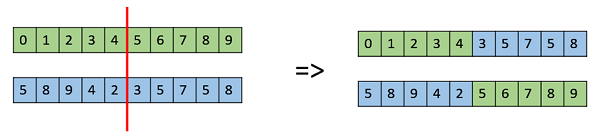
\includegraphics[scale = 0.85]{images/one_point_crossover.jpg}
    \caption{Single Point Crossover}
    \label{fig:crossover}
\end{figure}

The next core function was selection. The article cited they chose to used a form of tournament selection but did not explain how this occurred with the chromosomes \cite{bandyopadhyay_maulik_2002}. Tournament selection in our case, works with what we define as the proportional weights. We first applied our proportional weights to each centroid for ordering purposes. Given a centroid, $C_k$, its proportionate weight is its error to the relative fitness. In this case it would be $C_k$'s errors versus all the errors generated by all the centroids.\\ 

Now that we have established what the proportional weights for the system looks like with respects to centroids, we can now describe what our tournament selection is. Our selection would begin by ingesting two sets of chromosomes, taking the union of the two sets, and then it would be sorted by the proportionate weights from least to greatest. We would then begin the selection process by iterating through the sorted set. A selection probability would then be used to see if that particular element was used for the future generation as shown in equation (\ref{eq:selected}). 
\begin{equation}
select = p\cdot (1-p)^i
\label{eq:selected}    
\end{equation}
We let $p$ describe the proportional weight of element $i$ where $i$ is the index in the array of the sorted weights with a zero index. The reason why we chose to do it this way is because it preserves the centroids across the selection process. The selection will terminate when either the there is no more possible options to be selected or the array has selected $k$ centroids. If the former occurs then that would be an illegal states and the offspring would die off. If the latter occurs we have a new state. \\

The last function of mutation can either take the form of age-based mutation and offspring-based mutation. Age-based mutation occurs when a particular member of the gene pool is updated to reflect the assignments from the clustering process. We will select a member of the current generation and update the centroid chromosomes to reflect the assignments. The updating centroids process will occur with some probability $\gamma$. The offspring-based mutation would be purely exploratory because for each element in the chromosome array. Each chromosome has probability $\mu$ of being update by $\delta$ and $\epsilon$ where each are value between 0 and 1. The mutated chromosome would be modified by $\pm (\delta + \epsilon)$. To make our lives easier for deciding on what is a plus or a minus, we decided to assume both.  In this case, we generate two offsprings with mutation one where each element that was selected would be the plus case and one where the minus case. It is also worth noting that the selections of pluses and minuses are independent of each other to ensure a good mixing. That way there will not be one new offspring where each mutate chromosome has added values and one where something is subtracted.   \\

We can now describe the core algorithm where we first seed the algorithm with an initial gene pool. In most cases, we would choose the seeding pool to be 10-25 sets of chromosomes. We would then generate the next generation from the current generation of genes. This is where the basic functions come into play because these are how the next generations are produced. These functions will continue to be called until the number of future offsprings hit a desired amount signaling to move to the next generation. The algorithm will terminate when the $n^{\text{th}}$ generation is completed, we will look at the all the possible sets of chromosomes from the $n^{\text{th}}$  generation and select the best one.   
\section{Summary of Results} \label{sec:results}
\subsection{Quantifying Results}

There are three ways we chose to quantify the result of the data, the homogeneity score,  completeness score and the v-measure score. All three are indexing values that would range from 0.0 to 1.0. We chose these impartially because they are built into sklearn for quantifying cluster assignments with labeled data. The homogeneity score can be described as all value in an arbitrary cluster prediction comes from a singular label or category. Take for instance two parallel arrays,  one represents the actual labels, [0, 0, 1, 1], and the other represents the predicted values for the clustering,  [0, 0, 1, 2]. In this simple example the homogeneity score would be 1.0 because it is a near perfect mapping. \\

The completeness score goes in the opposite direction of the homogeneity score. Instead of seeing if the predicted values come from a singular truth partition, this scoring metric checks to see if the truth values are held together in the mapping process to the predicted labels. The example above would still have an indexing value of 0.66 because not all 1's in the truth array stayed together in the mapping. In this the second 1 is mapped to cluster 2 as opposed to cluster 1.  \\

The v-measurement score is just the harmonic mean of the homogeneity score and completeness score.  V-measurement scores will follow equation  (\ref{eq:v-measure}), where $HS$ is the homogeneity score and $CS$ is the completeness score.

\begin{equation}
\frac{2\cdot(HS \cdot CS) }{(HS + CS)}
\label{eq:v-measure}
\end{equation}
All three of these indexing values would be used to quantify the following results. 
\subsection{Types of Data}
\subsubsection{Simulated Data}
This dataset was built using a script to generate $k$-clusters of various size based on known distributions in $\mathbb{R}^2$.  The purpose was to test the algorithms to see what would come about in this simplified case with densely packed data.  This dataset also had the inherent benefit of being in $\mathbb{R}^2$ which allowed us the ability to plots the results.  We chose to have five distinct clusters for our test with over 1000 points.  The original clusters varied in size from 50 to 300 points. The results of  some of the clusters that formed could be seen in Figure \ref{fig:sim_plots} with the numerical results seen in Table \ref{tab:simulated}.
\begin{figure}[H]
   \centering
   \subfloat[][]{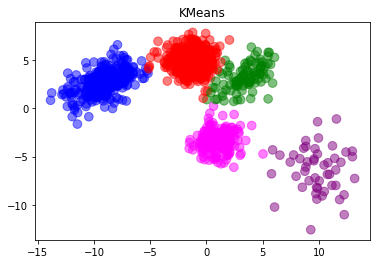
\includegraphics[width=.4\textwidth]{images/KMeans.png}}\quad
   \subfloat[][]{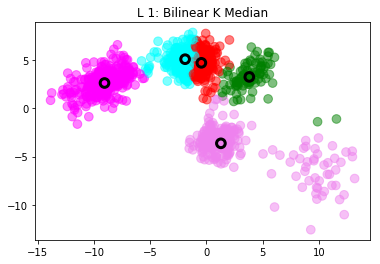
\includegraphics[width=.4\textwidth]{images/BilinearL1.png}}\\
   \subfloat[][]{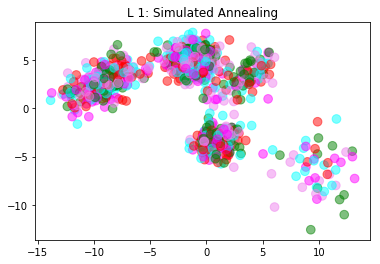
\includegraphics[width=.4\textwidth]{images/SA_L1.png}}\quad
   \subfloat[][]{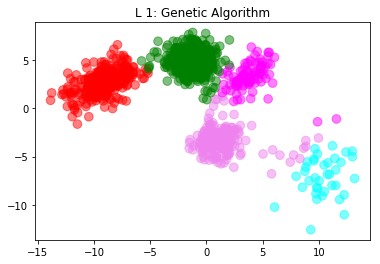
\includegraphics[width=.4\textwidth]{images/GeneticAlgorithmL1.png}}
   \caption{Clustering Plots for the Simulated Data}
     \label{fig:sim_plots}
\end{figure}

\begin{table}[H]
\centering
\caption{Simulated Data Result}\label{tab:simulated}
\begin{tabular}{|c|c|c|c|}
\hline
Algorithm                                                             & \begin{tabular}[c]{@{}c@{}}Homogeneity \\ Score\end{tabular} & \begin{tabular}[c]{@{}c@{}}Completeness\\ Score\end{tabular} & \begin{tabular}[c]{@{}c@{}}V-Measure\\ Score\end{tabular} \\ \hline
KMeans                   & 0.937        & 0.941    & 0.939                                                     \\ \hline
$\ell_1$:KMedian                                                          & 0.841                                                        & 0.742                                                        & 0.789                                                     \\ \hline
$\ell_\infty$: KMedian                                                        & 0.849                                                        & 0.739                                                        & 0.790                                                     \\ \hline
\begin{tabular}[c]{@{}c@{}}$\ell_1$:Simulated \\ Annealing\end{tabular}   & 0.674                                                        & 0.534                                                        & 0.596                                                     \\ \hline
\begin{tabular}[c]{@{}c@{}}$\ell_\infty$: Simulated \\ Annealing\end{tabular} & 0.671                                                        & 0.534                                                        & 0.596                                                     \\ \hline
\begin{tabular}[c]{@{}c@{}}$\ell_1$:Genetic \\ Algorithm\end{tabular}     & 1.00                                                         & 1.00                                                         & 1.00                                                      \\ \hline
\begin{tabular}[c]{@{}c@{}}$\ell_\infty$: Genetic \\ Algorithm\end{tabular}   & 1.0                                                          & 0.99                                                         & 0.99                                                      \\ \hline
\end{tabular}
\end{table}

In the case of the simulated data, it was interesting to see that the genetic algorithms for both $\ell_1$ and $\ell_\infty$ performed so well. The genetic algorithms were able to rebuild the original assignments of the data. We suspect that this is due to combination of the data being originally densely packed and being built using uniform distributions. Thus the genetic algorithm could find the distribution of the points. It is also worth noting how the results from the new algorithms were not incredibly different between the $\ell_1$ and $\ell_\infty$ case. 

\subsubsection{Iris Dataset}
This dataset comes from University of California Irvine's repository, it has 150 observations with 4 features in the reals. There were three distinct labels to describe the type of flower. For each of the algorithms, I asked for 4 clusters to be generated. The numerical results after running each dataset can be seen Table \ref{tab:iris}.
\begin{table}[H]
\centering
\caption{Iris Dataset Results}\label{tab:iris}
\begin{tabular}{|c|c|c|c|}
\hline
Algorithm                                                             & \begin{tabular}[c]{@{}c@{}}Homogeneity \\ Score\end{tabular} & \begin{tabular}[c]{@{}c@{}}Completeness\\ Score\end{tabular} & \begin{tabular}[c]{@{}c@{}}V-Measure\\ Score\end{tabular} \\ \hline
KMeans                                                               & 0.765                                                        & 0.751                                                        & 0.758                                                     \\ \hline
$\ell_1$:KMedian                                                          & 0.797                                                        & 0.794                                                        & 0.796            \\ \hline
$\ell_\infty$: KMedian                                                        & 0.797                                                        & 0.795                                                        & 0.796                                                     \\ \hline
\begin{tabular}[c]{@{}c@{}}$\ell_1$:Simulated \\ Annealing\end{tabular}   & 0.00157                                                        & 0.00156                                                        & 0.00157            \\ \hline
\begin{tabular}[c]{@{}c@{}}$\ell_\infty$: Simulated \\ Annealing\end{tabular} & 0.0325                                                        & 0.0324                                                        & 0.0324                                                     \\ \hline
\begin{tabular}[c]{@{}c@{}}$\ell_1$:Genetic \\ Algorithm\end{tabular}     & 0.7412                                                         & 0.728                                                         & 0.734                                       \\\hline                         
\begin{tabular}[c]{@{}c@{}}$\ell_\infty$: Genetic \\ Algorithm\end{tabular}   & 0.746                                                          & 0.743                                                         & 0.744                                                      \\ \hline
\end{tabular}
\end{table}
In this case, all the algorithms performed relatively the same except for simulated annealing algorithms. In this case,  we suspect it did poorly because of how we chose to generate potential new states. Since the new state generation is done purely randomly by selecting $\frac{2}{3}$ of the data to be adjusted to a new cluster it could be undoing any good choices that get generated. Also, since the data is not incredibly densely packed it could be causing some issues in the simulated annealing clustering algorithm.  
\subsubsection{Mushroom Dataset}
The last dataset comes from UCI as well, it has over 8000 observations of various mushrooms with 22 categorical features. Each observation is classified as either edible or poisonous. In this data, since it is purely categorical, we needed to transform it into 0 and 1 encoding for each categorical feature was reduced to. After using the OneHotTransaction function in sklearn, the number of features 117 that described if a feature can be applied to an observation. The results after applying each algorithm can be seen in Table \ref{tab:mushroom}. 
\begin{table}[H]
\centering
\caption{Mushroom Dataset Results}\label{tab:mushroom}
\begin{tabular}{|c|c|c|c|}
\hline
Algorithm                                                             & \begin{tabular}[c]{@{}c@{}}Homogeneity \\ Score\end{tabular} & \begin{tabular}[c]{@{}c@{}}Completeness\\ Score\end{tabular} & \begin{tabular}[c]{@{}c@{}}V-Measure\\ Score\end{tabular} \\ \hline
KMeans                                                                                                       & 0.347              & 0.662                                                     & 0.455                                                     \\ \hline
$\ell_1$:KMedian                                                          & 0.324                                                       & 0.602                                & 0.4212            \\ \hline
$\ell_\infty$: KMedian                                                        & 0.220                                                       & 0.263                                                        & 0.796                                                     \\ \hline
\begin{tabular}[c]{@{}c@{}}$\ell_1$:Simulated \\ Annealing\end{tabular}   
                                                     & $5.611 \cdot 10^{-5}$            & 0.000113                                                 & $7.58 \cdot 10^{-5}$            \\ \hline
\begin{tabular}[c]{@{}c@{}}$\ell_\infty$: Simulated \\ Annhnealing\end{tabular}                                                        & $5.611 \cdot 10^{-5}$      & 0.000113                                                   & $7.58 \cdot 10^{-5}$            \\\hline
\begin{tabular}[c]{@{}c@{}}$\ell_1$:Genetic \\ Algorithm\end{tabular}                                                     & 0.314           & 0.5596                                                & 0.403                                       \\\hline                         
\begin{tabular}[c]{@{}c@{}}$\ell_\infty$: Genetic \\ Algorithm\end{tabular}                                                         & 0.201        & 0.242     & 0.240                                                                                              \\ \hline
\end{tabular}
\end{table}

Categorical datasets are always interesting to try and cluster because the data is incredibly sparse. In this case the $\ell_\infty$ norm did much worse than the $\ell_1$ norm; we suspect it to be in part because of the style of data we are feeding the system. The $\ell_\infty$ norm is based on the max difference between the two vectors it probably could not determine how much improvement the new centroid locations were on the system. In particular it would only take one of the 117 features to be different from the centroid to produce a distance of 1. This is also a problem, for the assignment of points because the assignments are done in a greedy fashion; the $\ell_\infty$ norm would not be able to determine which centroids are necessarily better to the assignments.  This may not be a problem for categorical data in lower dimension but because we are over 100 spacial dimensions with only being 0 and 1 this could pose a problem. \\

The other thing, we should mention is that this dataset has a much larger number of observations than any of the others. We kept the genetic algorithm running with the same run parameters as the iris dataset. Since the mushroom dataset is so much larger than the Iris Dataset it should be worth mentioning what would happen if we increased the artificial section process. We could increase the number of generations for the model or increase the number of required offspring before going onto the next generation. That way the genetic algorithm would have results much closer to the bilinear case for at least the $\ell_1$ case.

\section{Future Work}
In terms of further work in this area there are two possible options that we discussed. The first would be looking at the weighted clustering models. In our current models, they only use the uniform case of clustering where each feature is weighted equally to the other features. In reality there would be features that would be more indicative of the desired output. Therefore, we could put more emphasis in that particular feature when building the clusters.  \\

The other problem to be further explored would be the topology of the system for clustering. Since clustering algorithms are seeding dependent, it would be interesting to look at how wide some of the areas of convergence for generating the clusters are. In this case the most common output of the clustering algorithm would be a very wide cup because multiple starting values will converge to that output. This particular output is a local minimum but the global minimum is could be a very skinny cup so it is very difficult to find these starting values. 

\bibliographystyle{acm}
\bibliography{citation}

\end{document}
